Após aplicar os métodos descritos, foram alcançados os seguintes resultados: a prototipação das telas para dispositivos móveis utilizando o Figma, a criação do site com o Oracle APEX, a elaboração do Diagrama de Caso de Uso (DCU), o Escopo de Redes, a modelagem relacional e lógica do banco de dados (MBD), e o desenvolvimento do Modelo de Negócios Canvas.

\textbf{Prototipação do aplicativo no Figma}

A \Cref{fig:splash-screen} mostra a tela de splash screen do projeto, tendo a logo, a paleta de cores da identidade visual e a escolha do modo de entrada ou cadastro. Após logar ou se cadastrar você será levado à tela do inicio. 

\begin{figure}[H]
\centering
\caption{Splash Screen}%
\label{fig:splash-screen}
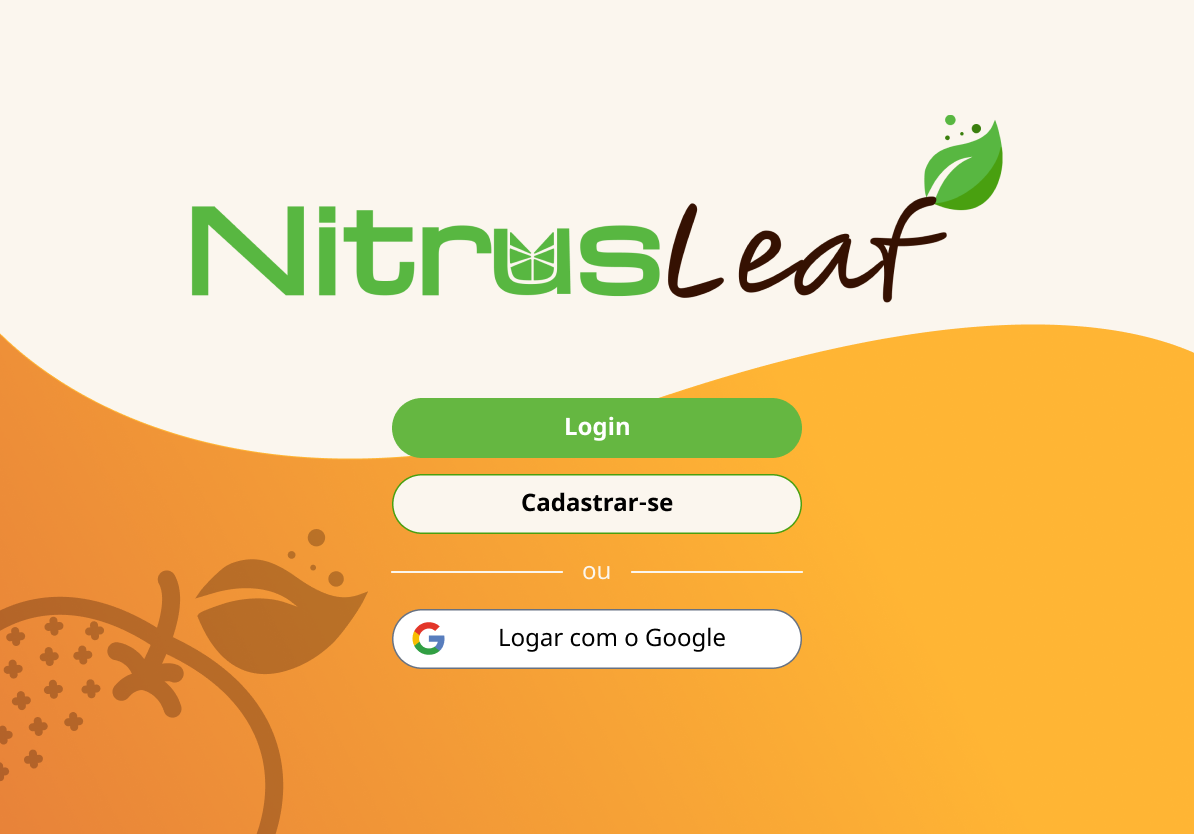
\includegraphics[width=0.8\linewidth]{Illustrations/Splash-Screen.png}
\SourceOrNote{Autoria Própria (2024)}
\end{figure}

A tela do inicio \Cref{fig:tela-inicio} oferece a opção de escanear a folha com o celular ou fazer o upload de uma imagem para escaneamento. Acima dessas duas opções encontra-se um quadrado contendo um gráfico de pizza que mostra a porcentagem da ocorrência das incidências, sendo amarelo manganês, laranja-avermelhado cobre e cinza adversos, que ocorre quando não há incidência de cobre nem de manganês. Um menu no canto esquerdo permite acessar outras telas do aplicativo, como histórico, drone e configurações gerais.

\begin{figure}[H]
\centering
\caption{Tela Início}%
\label{fig:tela-inicio}
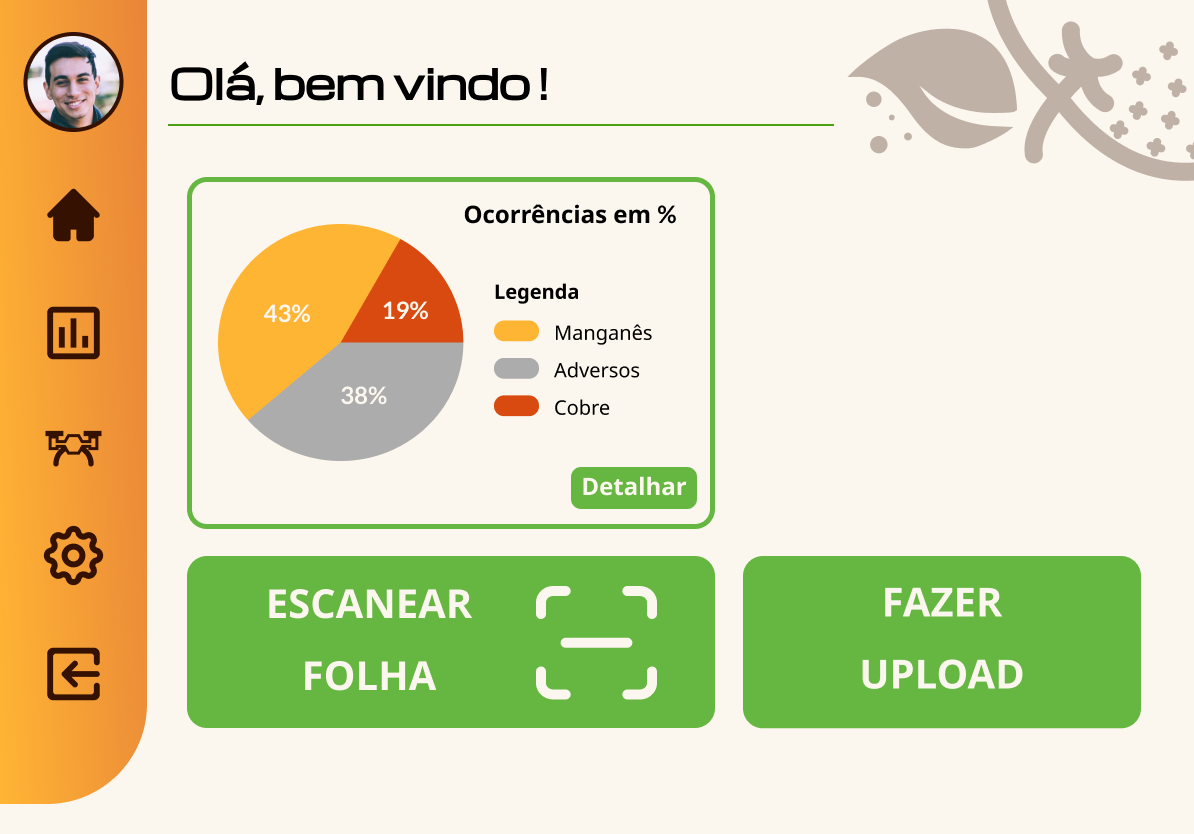
\includegraphics[width=0.8\linewidth]{Illustrations/tela-inicio.png}
\SourceOrNote{Autoria Própria (2024)}
\end{figure}

Ao apertar em escanear folha \Cref{fig:tela-escaneamento} será necessário apontar a câmera do celular para a folha escolhida e o aplicativo vai começar a escaneá-la e após terminar abrirá uma tela para você salvar a identificação da folha.


\begin{figure}[H]
\centering
\caption{Tela Escaneamento}%
\label{fig:tela-escaneamento}
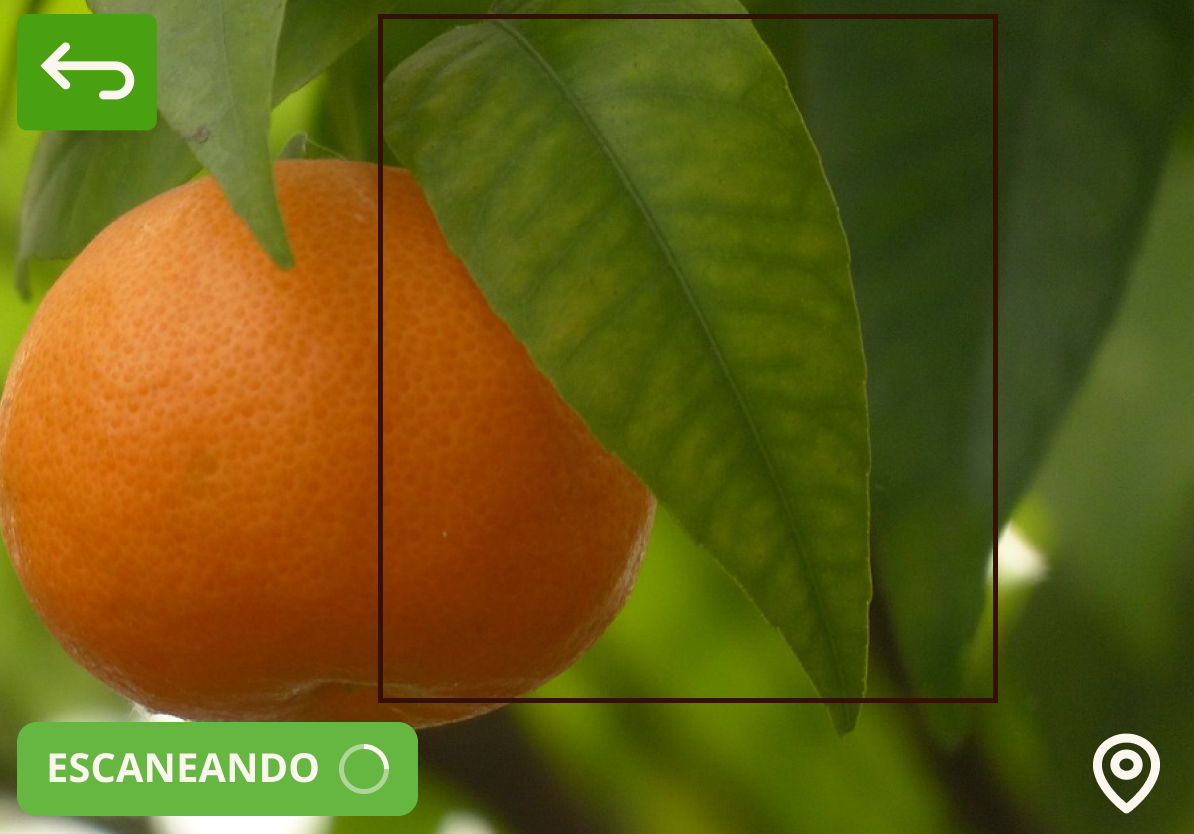
\includegraphics[width=0.8\linewidth]{Illustrations/Tela-Escaneamento.png}
\SourceOrNote{Autoria Própria (2024)}
\end{figure}

Após concluir o processo de escaneamento, o usuário será direcionado para uma tela onde poderá identificar o talhão correspondente à área escaneada, bem como o pé da folha que foi escaneada. Um talhão é uma área delimitada destinada ao plantio agrícola. Além disso, a tela mostrará a probabilidade de ser determinada uma deficiência, como ilustrado na \Cref{fig:cadastro-diagnóstico}. A opção de identificar da uma forma de controle para o usuário ter as informações de qual o pé que foi escaneado e o local em que ele foi escaneado salvas, possibilitando um maior controle para verificar se está tendo um grande número de incidências em um local específico.

\begin{figure}[H]
\centering
\caption{Cadastro Diagnóstico}%
\label{fig:cadastro-diagnóstico}
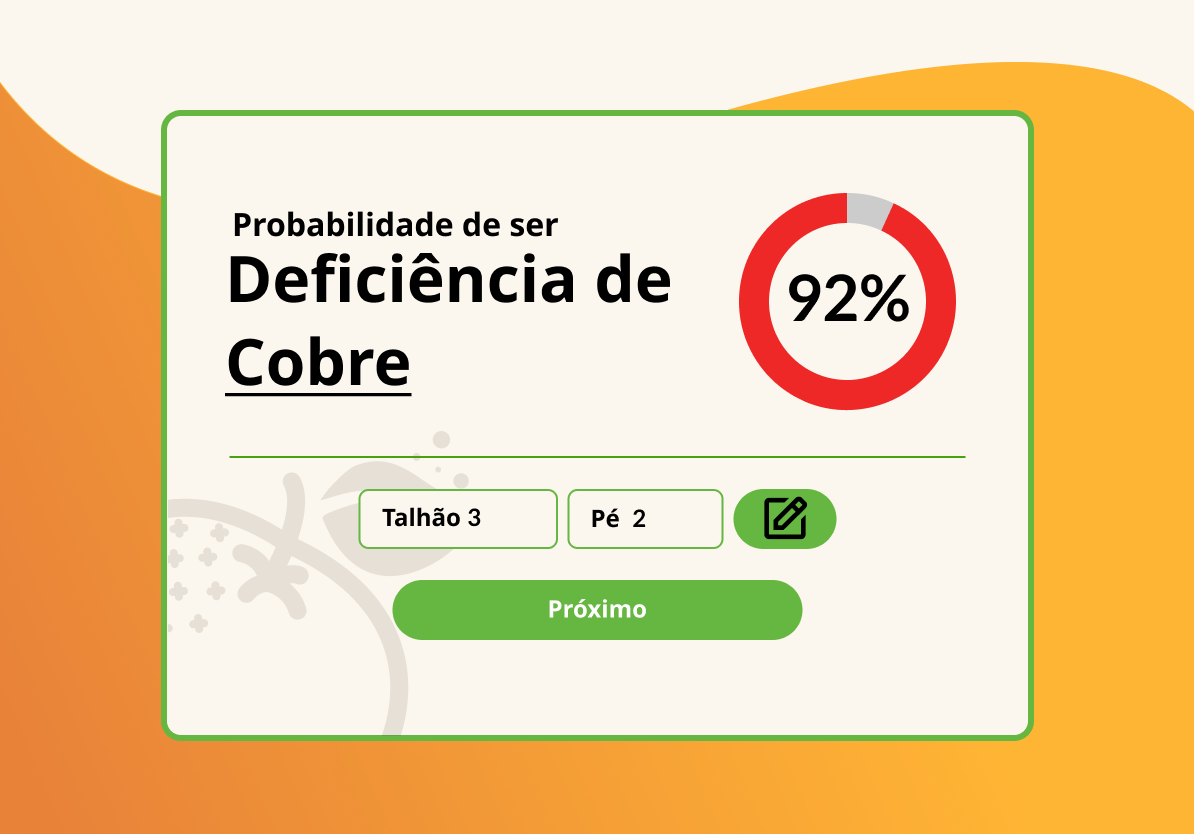
\includegraphics[width=0.8\linewidth]{Illustrations/Cadastro-diagnostico.png}
\SourceOrNote{Autoria Própria (2024)}
\end{figure}

Também a a tela com as informações tiradas dos drones \Cref{fig:tela-drone}, que seria o Índice de  estado de vegetação (NDVI) que é criado pelo drone ao tirar uma foto do local escolhido e um gráfico de linhas mostrando o nível do NDVI de cada talhão ao longo de 12 meses. O NDVI visa medir a quantidade de energia refletida e absorvida pelas plantas, fornecendo informações sobre sua saúde com base nessa reflectância. Na planta a parte de energia que é absorvida é o espectro da luz visível que vai de 400 a 720 nm (nanômetros), a parte que não é absorvida é a do espectro infravermelho próximo a luz visível, 720 a 1100 nm. As plantas saudáveis absorvem boa parte da luz visível e refletem fortemente o infravermelho próximo a luz visível. Já uma planta que está desidatrada, sofrendo de alguma doença ou algo que afete a sua saúde, absorvera mais da luz infravermelha. Logo o NDVI verificará a saúde das plantas por meio da refletividade das plantas. E de acordo com esse conhecimento terá uma fórmula que utilizará dos espectros que a planta reflete e absorve, (NIR) como a refletividade do infravermelho próximo e (VIS) como a refletividade vermelha. A fórmula é NIR menos o VIS dividido por NIR mais o VIS \cite{ResultadoNDVIArtigo, ResultadoNDVISite}.  

\[ NDVI =  \frac{NIR - VIS}{NIR + VIS} \]

A partir dessa fórmula, é obtido o valor do NDVI, que varia de -1 a 1. Variações com pequenos valores, como por exemplo os valores negativos, são geralmente associados a corpos d'água, enquanto valores acima de zero, que estão próximos dos valores negativos, representam nuvens. Os valores acima de 0,4 indicam a saúde das plantas, sendo os valores entre 0,6 e 0,8 considerados como representativos de plantas saudáveis. Essas informações são apresentadas na legenda na tela do mapeamento do drone.

\begin{figure}[H]
\centering
\caption{Tela Drone}%
\label{fig:tela-drone}
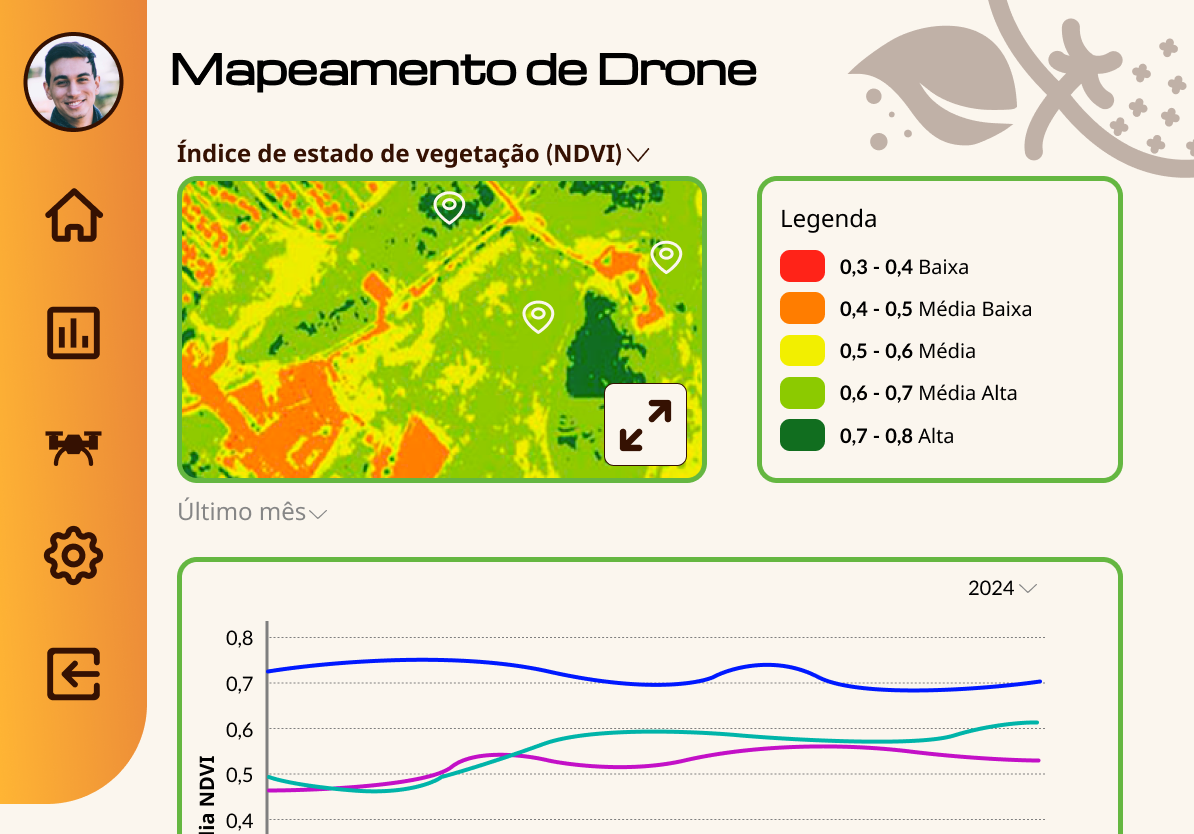
\includegraphics[width=0.8\linewidth]{Illustrations/tela-drone.png}
\SourceOrNote{Autoria Própria (2024)}
\end{figure}

Para verificar os pés cadastrados no aplicativo, acesse a tela de histórico \Cref{fig:tela-relatorios}. Nessa tela, você pode ver quantos pés estão cadastrados em cada talhão, bem como quantos pés do talhão foram analisados até o momento. No lado direito do histórico, uma janela de registros exibe o número total de talhões e pés registrados, assim como o número de pés analisados e diagnosticados.

\begin{figure}[H]
\centering
\caption{Tela Relatórios}%
\label{fig:tela-relatorios}
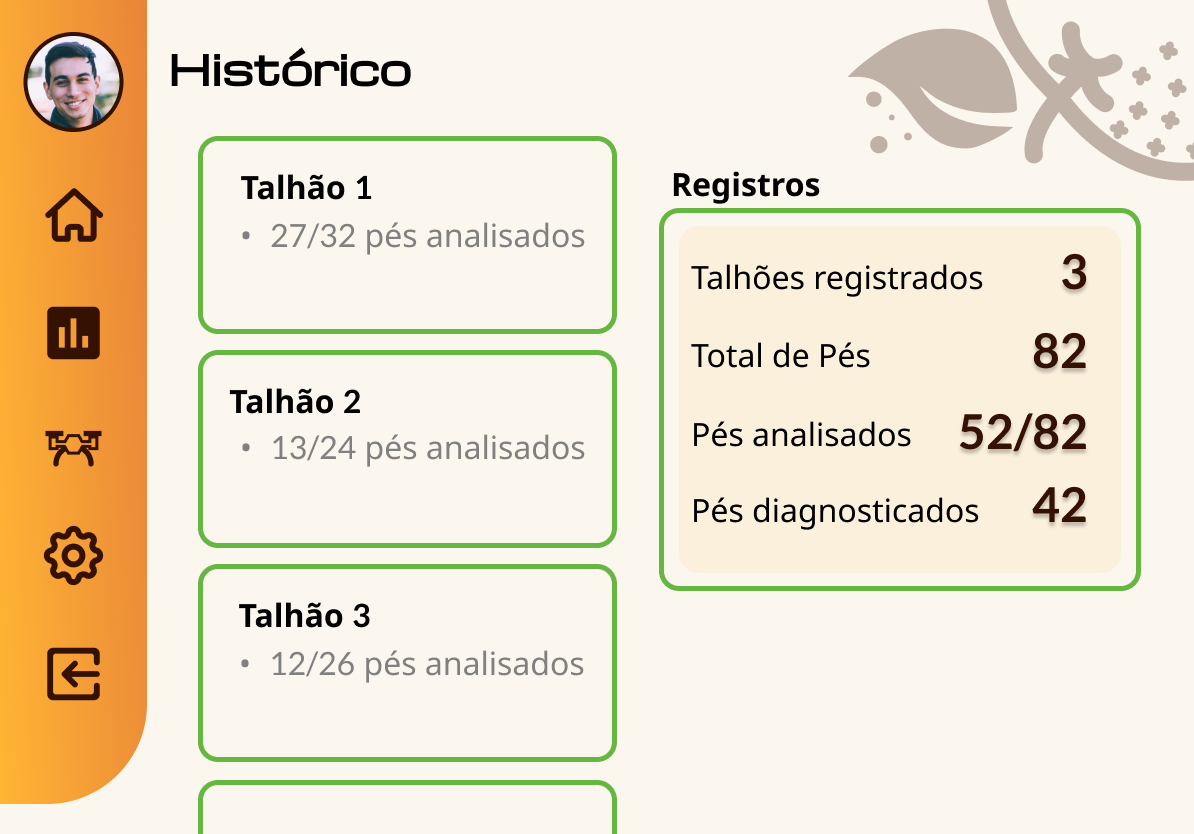
\includegraphics[width=0.8\linewidth]{Illustrations/tela-relatorios.png}
\SourceOrNote{Autoria Própria (2024)}
\end{figure}

\textbf{Oracle APEX}

Na aplicação desenvolvida no Oracle APEX, existem três telas principais. A primeira delas é a tela com o mapa, conforme ilustrado na \Cref{fig:APEX-mapa}. Esta tela exibe a localização exata de cada pé dentro dos talhões, fornecendo informações detalhadas sobre a incidência de condições, como deficiência de cobre, deficiência de manganês, ou nenhuma das duas, e identificando qual pé específico está sendo afetado.

\begin{figure}[H]
\centering
\caption{APEX Mapa}%
\label{fig:APEX-mapa}
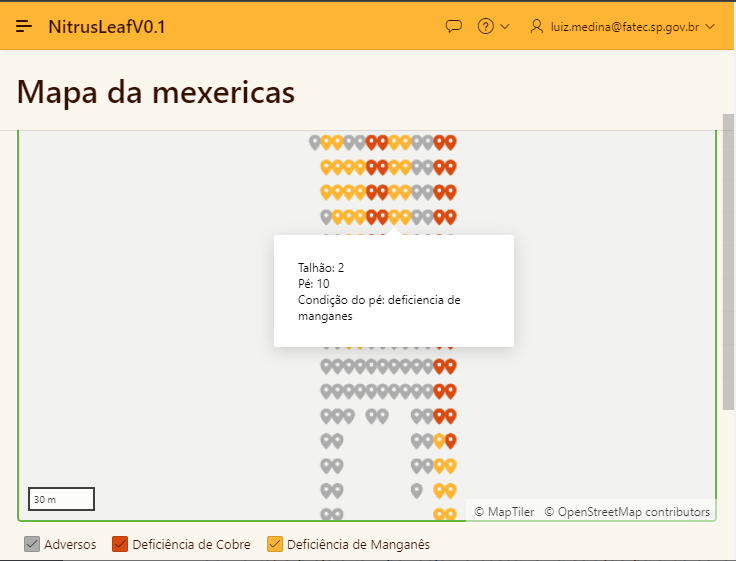
\includegraphics[width=0.8\linewidth]{Illustrations/mapa.png}
\SourceOrNote{Autoria Própria (2024)}
\end{figure}

A segunda tela da aplicação é a tela do mapa de calor, conforme ilustrado na \Cref{fig:APEX-mapa-de-calor}. Esta tela mostra a cor que identifica cada tipo de incidência e o nome correspondente. A concentração das cores aumenta conforme a proximidade das incidências. Por exemplo, se houver muitos casos de deficiência de manganês, eles estarão mais visíveis no mapa, permitindo a fácil identificação de grandes concentrações de deficiências nos locais.

\begin{figure}[H]
\centering
\caption{APEX Mapa de calor}%
\label{fig:APEX-mapa-de-calor}
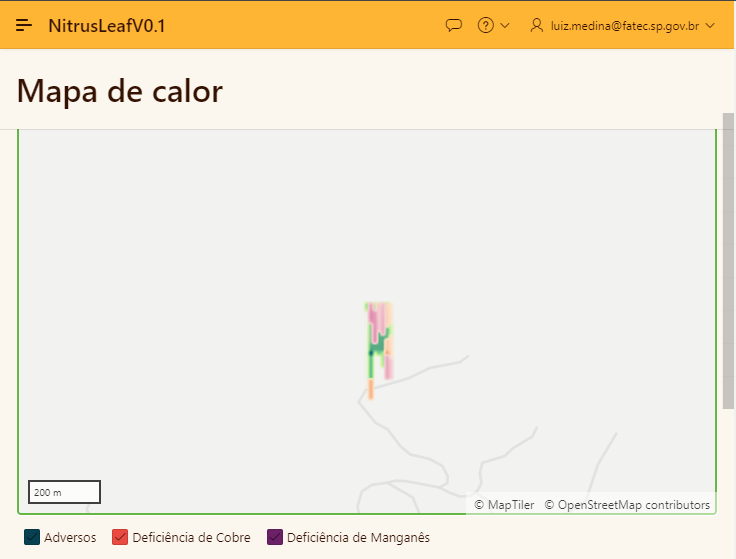
\includegraphics[width=0.8\linewidth]{Illustrations/mapadecalor.png}
\SourceOrNote{Autoria Própria (2024)}
\end{figure}

A última tela é a tela dos gráficos, conforme ilustrado na \Cref{fig:grafico}. Há dois gráficos: um gráfico de barras mostrando o número total de cada incidência e o número de pés que não apresentaram nenhuma das duas deficiências, categorizados como Adversos. O segundo gráfico é um gráfico de pizza, mostrando a porcentagem de cada incidência e a proporção de pés que não apresentam nenhuma das deficiências.

\begin{figure}[H]
\centering
\caption{APEX Gráficos}%
\label{fig:grafico}
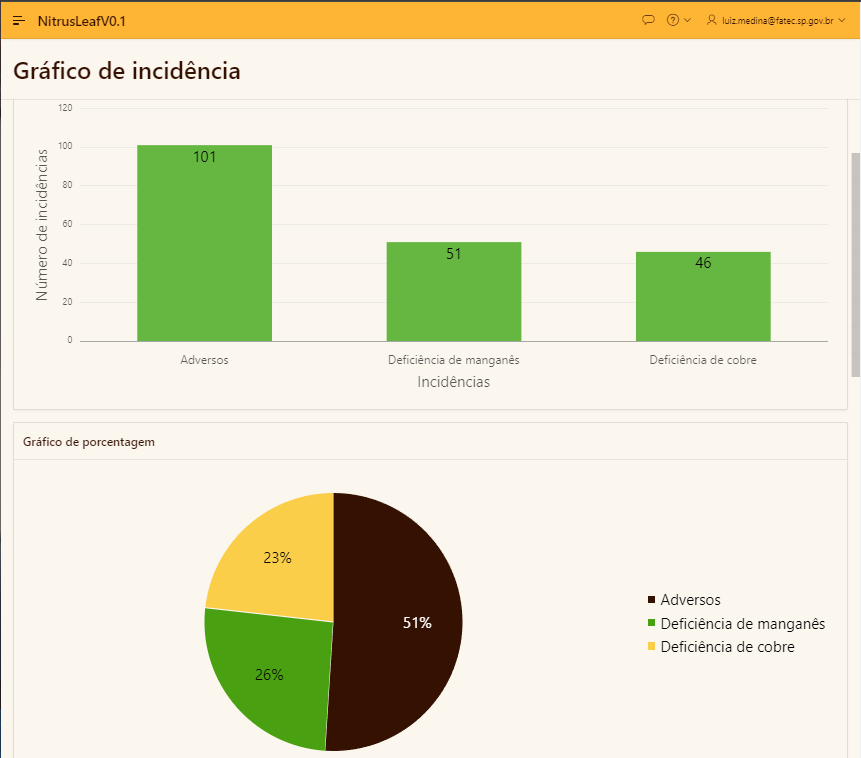
\includegraphics[width=0.8\linewidth]{Illustrations/grafico.png}
\SourceOrNote{Autoria Própria (2024)}
\end{figure}

\textbf{Diagrama de caso de uso (DCU)}

O DCU do projeto, ou Diagrama de Caso de Uso, é um diagrama utilizado para explicar as relações entre os atores (utilizadores do sistema) e as funcionalidades disponibilizadas pelo projeto. Conforme ilustrado na \Cref{fig:dcu}, ele mostra que o proprietário deve cadastrar as mexeriqueiras e, se desejar, cadastrar os drones. O funcionário é responsável por escanear as folhas, podendo fazer isso tanto com a câmera quanto fazendo upload das imagens. O aplicativo fornecerá o diagnóstico baseado nas imagens. Além disso, o funcionário pode consultar o mapa NDVI gerado pelo drone, bem como consultar o histórico e visualizar estatísticas. As funções do drone incluem tirar fotos do local e enviar um mapa NDVI.



\begin{figure}[H]
\centering
\caption{Diagrama de caso de uso (DCU)}%
\label{fig:dcu}
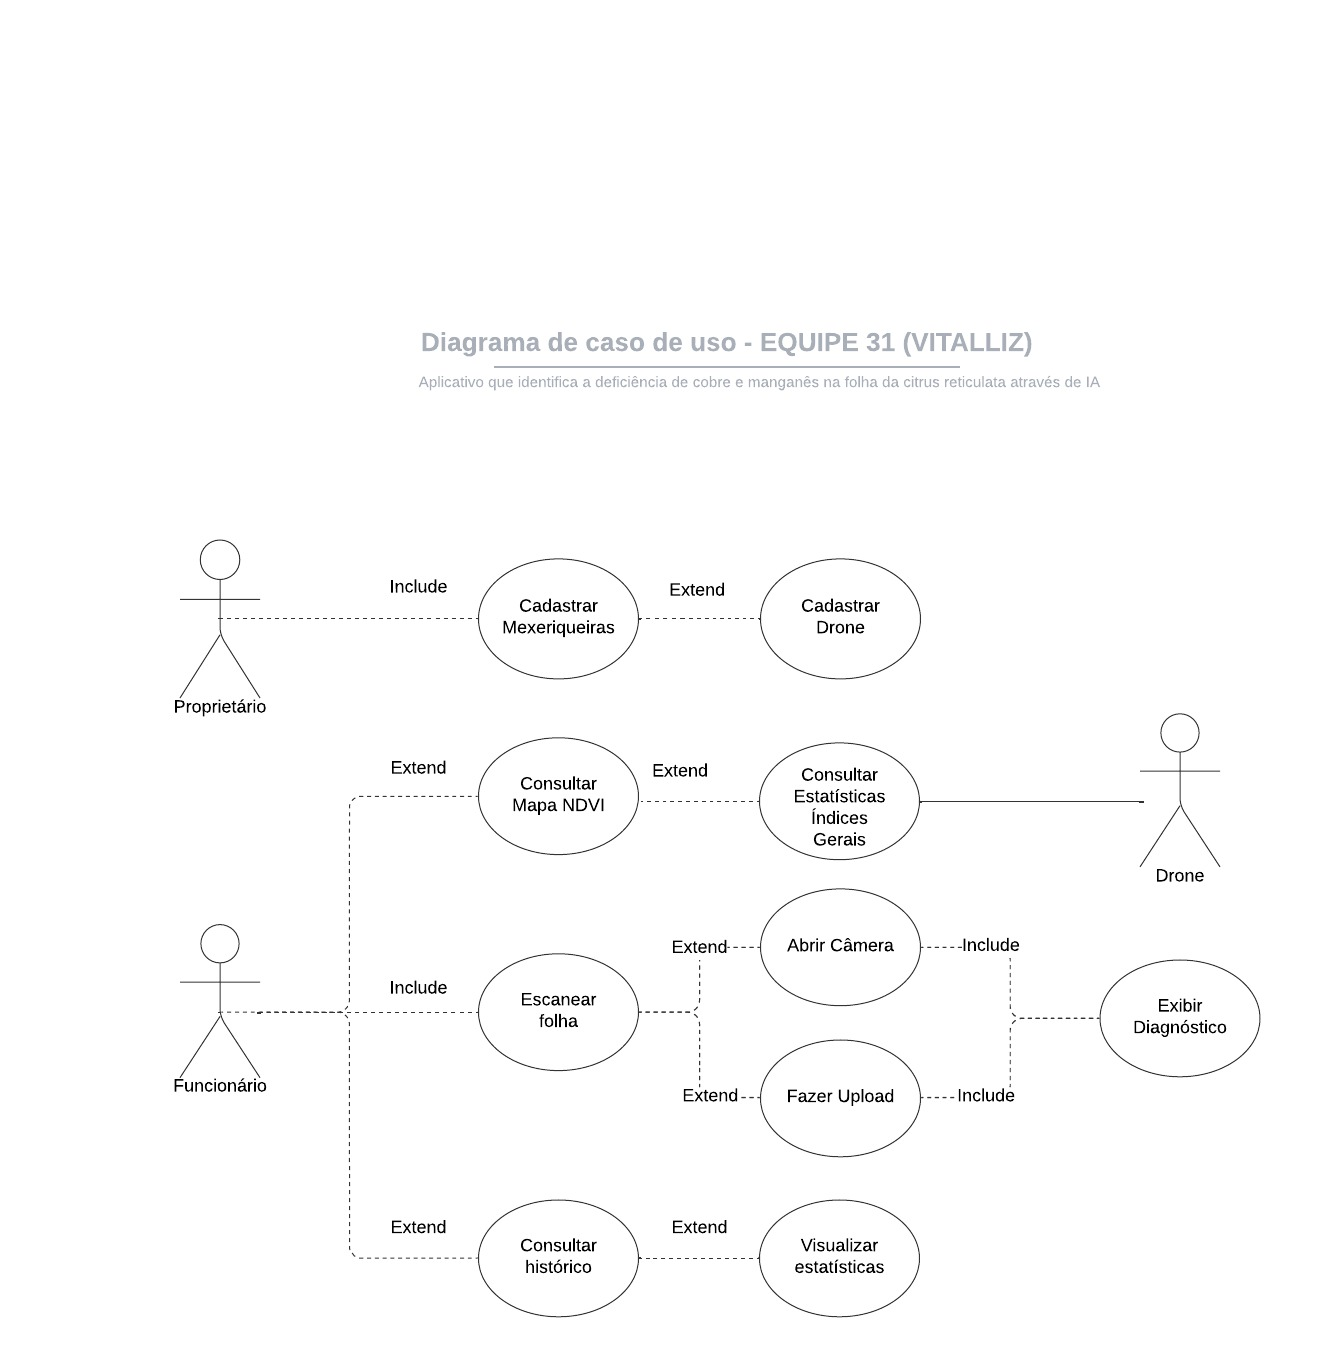
\includegraphics[width=0.8\linewidth]{Illustrations/dcu.jpeg}
\SourceOrNote{Autoria Própria (2024)}
\end{figure}

\textbf{Escopo de Redes}

A representação das ligações de rede do projeto é mostrada no escopo de redes, conforme ilustrado na \Cref{fig:escopoderedes}. Esta figura demonstra onde os programas são desenvolvidos e mantidos, sua conexão com a internet e o servidor, e a conexão do usuário com a internet. Quando o usuário envia fotos, estas passam pela internet e são armazenadas no servidor, que guarda as informações no banco de dados.

Os computadores estão todos conectados a um switch, que os conecta a um roteador. O roteador, por sua vez, os conecta à internet e, consequentemente, ao servidor. O roteador está localizado na área de manutenção.

Há também uma recepção, equipada com uma mesa para atender possíveis clientes. Nesta mesa, há um notebook conectado à internet via Wi-Fi, por meio de um modem com Wi-Fi que está situado na recepção.

\begin{figure}[H]
\centering
\caption{Escopo de Redes}%
\label{fig:escopoderedes}
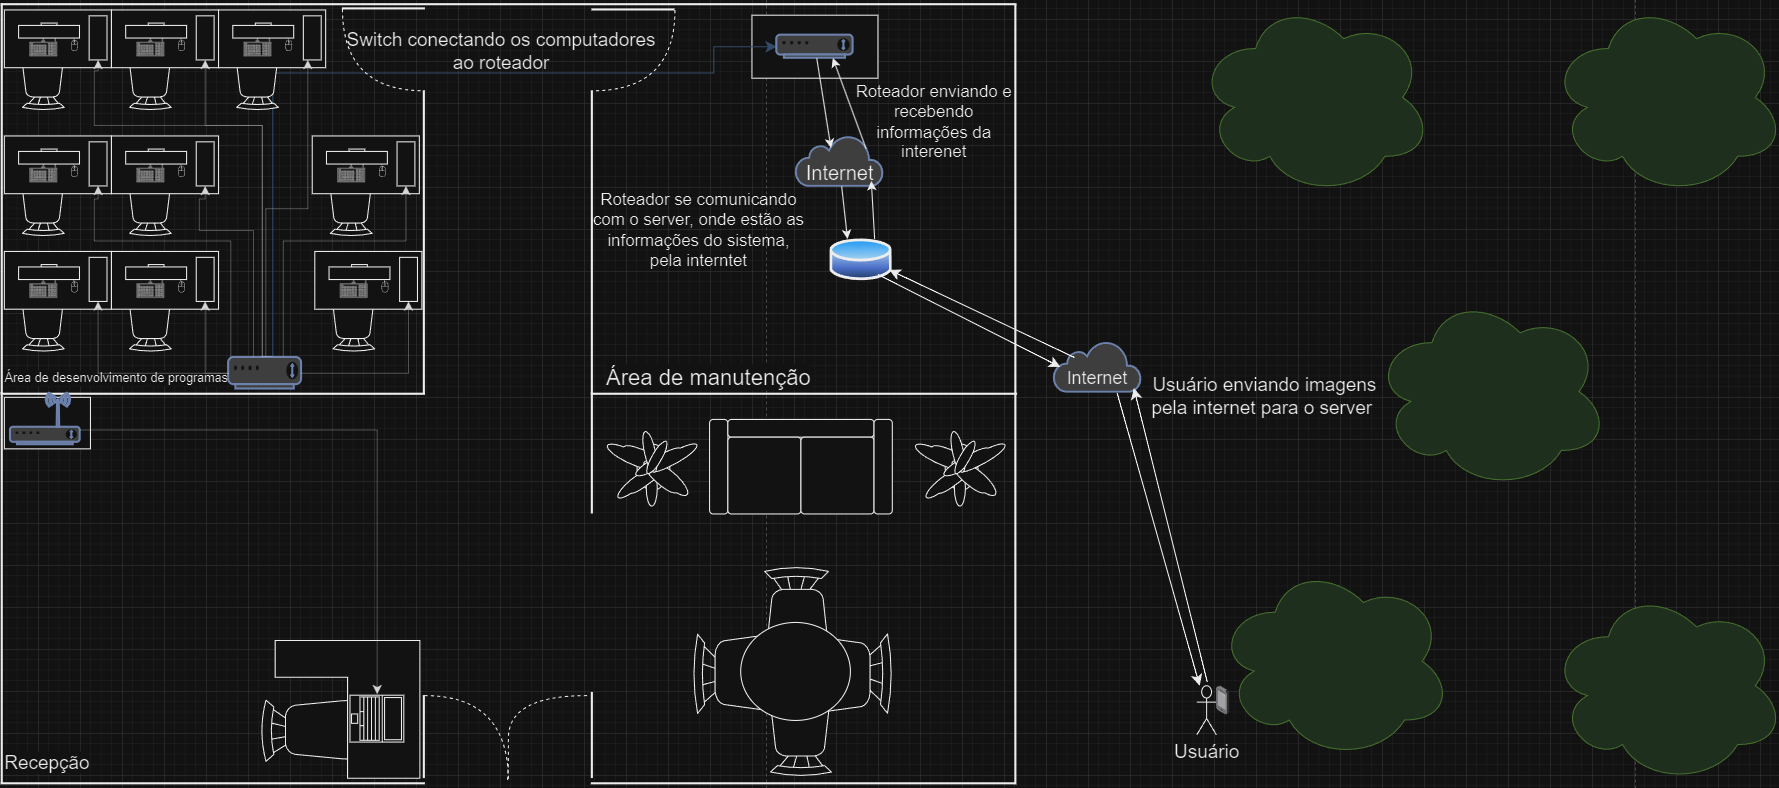
\includegraphics[width=0.8\linewidth]{Illustrations/escopoderedes.png}
\SourceOrNote{Autoria Própria (2024)}
\end{figure}

\textbf{Modelagem relacional e lógica do banco de dados}

A modelagem relacional do banco de dados \Cref{fig:mbdrelacional} do projeto NitrusLeaf tem como principal objetivo explicar a estrutura de dados utilizada para identificar deficiências nutricionais em folhas de mexeriqueira (Citrus reticulata). Este banco de dados é composto por várias entidades e seus respectivos relacionamentos, garantindo a integridade e a eficiência no armazenamento e consulta dos dados.

A entidade \textit{Folha} contém os atributos Id Fruta, Coloração Folhas, Tamanho e Nervuras, além de poder possuir três tipos de deficiência: manganês, cobre ou nenhuma deficiência. A entidade \textit{Foto} é considerada uma entidade fraca, utilizada para ligar a entidade \textit{Drone} e \textit{Folha}. \textit{Foto} possui os atributos Id\_Foto, Fk Id\_Drone (chave estrangeira que faz referência o drone), e Fk\_Id\_Fruta (chave estrangeira que referencia a folha).

A entidade \textit{Drone} tem os atributos Id\_Drone, Visibilidade, Qualidade e Capacidade. \textit{Drone} é responsável por gerar a entidade \textit{Imagem}, que possui os atributos Id\_Imagem, fk\_id\_Drone, Nitidez e Visibilidade. \textit{Imagem} é utilizada para identificar a coloração da folha através da entidade \textit{Coloração} e também gera a entidade \textit{Diagnóstico}. \textit{Diagnóstico} possui os atributos Id\_Diagnóstico, Fk\_Id\_Imagem (chave estrangeira que faz referência a imagem) e Qtd\_Historico. Em seguida, \textit{Diagnóstico} gera a entidade \textit{Histórico}, que contém os atributos Id\_Histórico, Data\_Emissão e Capacidade\_Armazem.

A entidade \textit{Imagem x Produtor} serve para relacionar a imagem com o produtor, possuindo os atributos Id\_ImgXProd, Fk\_Id\_Imagem e Fk\_Id\_Produtor. A entidade \textit{Produtor} tem os atributos Id\_Produtor e Nome, e interage com as entidades \textit{Email}, \textit{Telefone} e \textit{Login}. \textit{Email} possui os atributos Id\_Email, Fk\_Id\_Produtor e Correio\_eletrônico. \textit{Telefone} contém os atributos Id\_Telefone, Fk\_Id\_Produtor e Número, permitindo que o produtor tenha múltiplos números de contato. Por fim, a entidade \textit{Login} possui os atributos Id\_Login, Usuário e Senha.

Esse modelo relacional detalha como o banco de dados é estruturado para garantir a gestão eficiente das informações no aplicativo NitrusLeaf. Ele permite a identificação precisa de deficiências nutricionais nas folhas de mexeriqueira, suportando as funcionalidades do aplicativo, desde a captura de fotos pelos drones até a geração de diagnósticos e armazenamento de históricos. A estrutura relacional assegura que as informações sejam bem organizadas e facilmente acessíveis, otimizando o processo de recuperação das plantas e ajudando os produtores a evitar a perda de frutos. Além do modelo relacional, também há o modelo lógico mostrado na \Cref{fig:mbdlogico}.


Esse modelo relacional detalha como o banco de dados é estruturado para garantir a gestão eficiente das informações no aplicativo NitrusLeaf. Ele permite a identificação precisa de deficiências nutricionais nas folhas de mexeriqueira, suportando as funcionalidades do aplicativo, desde a captura de fotos pelos drones até a geração de diagnósticos e armazenamento de históricos. A estrutura relacional assegura que as informações sejam bem organizadas e facilmente acessíveis, otimizando o processo de recuperação das plantas e ajudando os produtores a evitar a perda de frutos. Além do modelo relacional, também há o modelo lógico mostrado na \Cref{fig:mbdlogico}.

\begin{figure}[H]
\centering
\caption{Modelo Relacional do Banco de Dados}%
\label{fig:mbdrelacional}
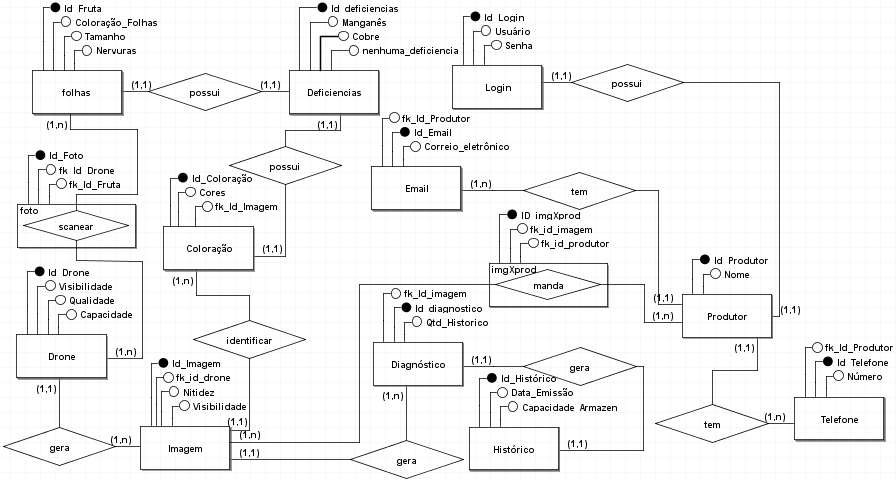
\includegraphics[width=0.8\linewidth]{Illustrations/mbdrelacional.png}
\SourceOrNote{Autoria Própria (2024)}
\end{figure}

\begin{figure}[H]
\centering
\caption{Modelo Lógico do Banco de Dados}%
\label{fig:mbdlogico}
\includegraphics[width=0.8\linewidth]{Illustrations/mbdlógico.png}
\SourceOrNote{Autoria Própria (2024)}
\end{figure}

\textbf{Modelo de negócios Canvas}

O modelo de negócios Canvas do projeto NitrusLeaf \Cref{fig:canvaspi} tem como principal objetivo delinear os elementos cruciais para o sucesso do nosso empreendimento. Esse modelo abrange várias áreas essenciais, incluindo nossos parceiros, proposta de valor, relacionamento com o cliente, recursos e atividades chave, canais, estrutura de custos e fontes de renda.

Parceiros Chave

Nosso foco principal em parceiros chave são os locais e entidades envolvidas no setor agrícola, especialmente aqueles interessados em inovação tecnológica. Esses parceiros incluem cooperativas agrícolas, universidades, centros de pesquisa, empresas de tecnologia agrícola, secretarias de agricultura dos municípios do Vale do Ribeira e associações de fazendeiros. A colaboração com esses parceiros é fundamental para ampliar o alcance do projeto e assegurar suporte técnico e científico.

Proposta de Valor

A proposta de valor do NitrusLeaf gira em torno da capacidade de identificar deficiências nutricionais nas plantas, especificamente a falta de manganês e cobre nas folhas de mexerica, de maneira eficiente e em tempo real. Além disso, o projeto visa manter um padrão elevado de qualidade dos frutos, ajudando os agricultores a otimizar a saúde das plantas e a produtividade.

Relacionamento com o Cliente

O relacionamento com o cliente é focado em oferecer um suporte abrangente. Isso inclui suporte técnico para a utilização do aplicativo via WhatsApp e feedback do cliente pelo app, além de canais de comunicação para feedback e resolução de dúvidas. Nosso objetivo é garantir que os clientes se sintam apoiados e possam maximizar os benefícios do nosso sistema.

Recursos Chave

Os recursos chave para o desenvolvimento e operação do NitrusLeaf incluem infraestrutura tecnológica (servidores, drones, câmeras de alta resolução), conhecimento técnico em agronomia e TI, uma equipe de suporte dedicada, programadores, instaladores do sistema físico, funcionários para suporte online e host para hospedar o site. Esses recursos são essenciais para o funcionamento eficaz do sistema.

Atividades Chave

As atividades chave do projeto incluem o desenvolvimento contínuo do software, a calibração dos algoritmos de IA para identificar deficiências nutricionais, a manutenção dos drones e outros equipamentos, e a realização de testes de campo para validar os diagnósticos fornecidos pelo sistema.

Canais

Os canais através dos quais promovemos e oferecemos nossos serviços incluem nosso website, redes sociais, feiras agrícolas, eventos de tecnologia, newsletters, parcerias com distribuidores agrícolas e anúncios pelas secretarias de agricultura dos municípios do Vale do Ribeira.

Estrutura de Custos

A estrutura de custos engloba despesas com desenvolvimento e manutenção do software, compra e manutenção de equipamentos (drones e câmeras), marketing e promoção, salários da equipe, custos operacionais gerais como servidores e infraestrutura de TI, manutenção dos itens que realizam o monitoramento das mexericas, compra dos produtos necessários para o monitoramento, host para hospedar as informações, aluguel do sistema e itens necessários, e mão de obra para instalação e manutenção.

Fontes de Renda

A principal fonte de renda do NitrusLeaf provém da venda de assinaturas para o uso do aplicativo, serviços de análise de solo e plantas, consultoria técnica, parcerias com empresas e aluguel do sistema.

Em resumo, o modelo de negócios Canvas do NitrusLeaf oferece uma visão abrangente de como estruturamos nosso projeto para atingir nossos objetivos e atender às necessidades dos nossos clientes. Nossa abordagem integrada garante que todos os aspectos do negócio estejam alinhados para promover a saúde e produtividade das plantações de nossos usuários.